\chapter{�bersicht Gesamtsystem}
\label{sec:teil1_uebersicht}

Das System besteht aus einem Smart Meter (EM340) und einem Gateway, auf welchem die Software zur Verbrauchsanalyse installiert ist. Die Ger�te sind alle an der Phase L1 des Energiez�hlers angeschlossen. Prinzipiell ist der hier verwendete Energiez�hler  zwar so konzipiert, dass er auf drei verschiedenen Phasen Messungen durchf�hren k�nnte, in diesem Projekt wurde aber auschliesslich die Phase L1 genutzt.

TODO: Grafik SIOT erg�nzen 

\begin{figure}[H]
	\centering
	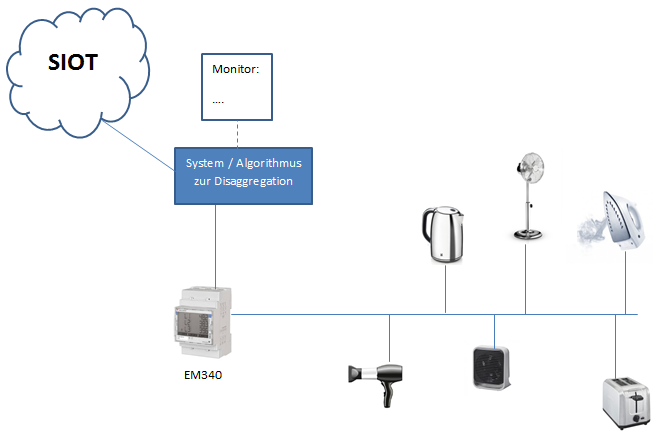
\includegraphics[width=1.0\textwidth]{Bilder/uebersicht.png} %70% der Textbreite
	\caption{�bersicht Gesamtsystem}
	\label{fig:teil1_pestle}
\end{figure}

Als Gateway dient hier ein Raspberry Pi, auf welchem das in Python geschriebene Programm l�uft,mit welchem die Daten aus dem Z�hler gelesen, verarbeitet und an das SIOT gesendet werden. Der Energiez�hler stellt verschiedene Register bereit, aus welchen jeweils pro Phase der Stromverbrauch I [A], die Spannung U [V], die Wirk P [W]-, Schein S [VA]- und Blindleistung Q [var] herausgelesen werden k�nnen. Diese Werte bilden die Grundlage zur Signaturerstellung der einzelnen Verbraucher.

\chapter{Erstellen von Signaturen der Verbraucher}
\label{sec:teil1_uebersicht}
Aufgrund der physikalischen Gegebenheiten beeinflusst jedes Haushaltsger�t Strom und Spannung auf unterschiedliche weise. Genauer gesagt unterscheidet man zwischen ohmschen-, kapazitiven- und induktiven Verbrauchern. Ohmsche Verbraucher bestehen aus einem oder mehreren Widerst�nden, d.h. elektrischen Komponenten, die im wesentlichen Hitze oder Licht erzeugen. Beispiele daf�r sind der Ofen, Gl�hbirnen oder B�geleisen. Beim rein ?ohmschen? Verbraucher (dem ohne induktiven oder kapazitiven Anteil) sind Spannung und Strom stets ?in Phase?, d.h. es gibt keine Phasenverschiebung und somit keinen Blindleistungsanteil, was gleichzeitig auch bedeutet, dass die Wirkleistung gleich der Scheinleistung entspricht. Induktive Verbraucher sind im wesentlichen elektromagnetische Verbraucher, d.h. elektrische Komponenten, die Elektromagnetismus erzeugen. Diese Ger�te ben�tigen beim Anlauf unter Umst�nden ein vielfaches an Anlaufstrom. Beispiele daf�r sind Pumpen oder auch Ventilatoren. Bei rein induktiven Komponenten eilt die Spannung dem Strom voraus, wodurch sich eine Phasenverschiebung von 90 Grad ergibt. D.h. hier gibt es einen Blindleistungsanteil und somit ist die Wirkleistung ungleich der Scheinleistung. Kapazitive Verbraucher verhalten sich �hnlich wie induktive Verbraucher, mit dem unterschied, dass hier keine Magnetfelder aufgebaut werden, sondern elektrische Felder. Bei kapazitiven Lasten eilt der Strom der Spannung voraus, wobei auch hier wieder eine Phasenverschiebung von 90 Grad entsteht. D.h. also, dass auch kapazitive Lasten einen Blindleistungsanteil besitzen und die Wirkleistung nicht der Scheinleistung entspricht. Allerdings sind rein ohmsche, kapazitive und induktive Verbraucher eher selten und Misch-Verbraucher die Regel. D.h. also dass jeder Verbraucher in unterschiedlicher Weise Wirk-, Blin-, und Scheinleistung beeinflusst. Somit k�nnten zwei Verbraucher mit gleicher Wirkleistung trotzdem unterschieden werden aufgrund unterschiedlicher Blindleistungsanteilen. 

TODO: Grafiken induktiv, kapazitiv, ohmsche aus Wiki

Um f�r jedes Haushaltsger�t eine Signatur erstellen zu k�nnen, werden die Ger�te zu Beginn jeweils einzeln an das Smartmeter angeschlossen und die jeweiligen Register �ber einen Zeitraum von 30 Sekunden ausgelesen. Die so gewonnenen Daten werden anschliessend in einer Datenbank abgespeichert und einem Ger�t eindeutig zugewiesen. Diese Signatur wird dann schlussendlich verwendet um den Gesamtstromverbrauch auf die einzelnen Verbraucher aufschl�sseln zu k�nnen. F�r diess Projekt 2 Arbeit kamen folgende Haushaltsger�te zum Einsatz: Haarf�hn, Heizl�fter, Ventilator, B�geleisen, Toaster, Wasserkocher und Stabmixer. Die erstellten Signaturen werden auf folgenden Abbildungen illustriert. 

TODO: 3 Beispielgrafiken (Wasserkocher und tbd)
\chapter{Einleitung}
\label{chap:teil1_einleitung}\chapter{Einleitung}
\label{chap:teil1_einleitung}

\begin{figure}[H]
	\centering
	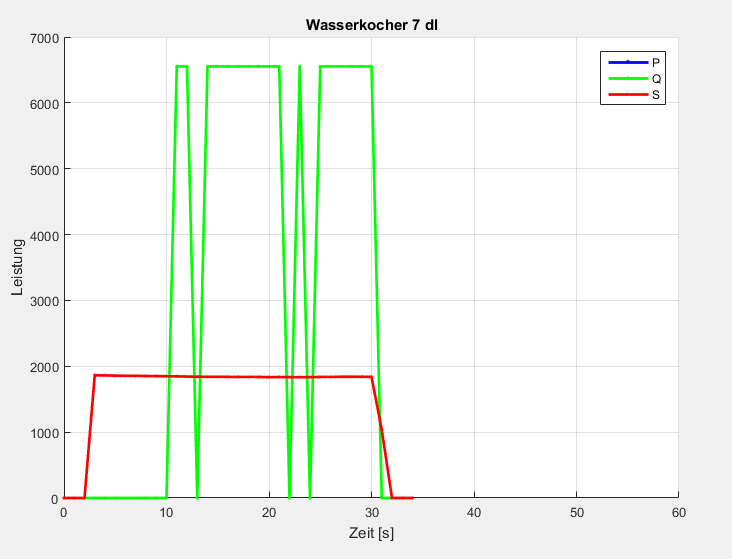
\includegraphics[width=0.5\textwidth]{Bilder/wasserkocher.png} %70% der Textbreite
	\caption{�bersicht Gesamtsystem}
	\label{fig:teil1_pestle}
\end{figure}

\chapter{Disaggregation: Ansatz mittels Kombinatorik}
\label{sec:teil1_kombinatorik}
-Algorthmus beschreiben (Inputs, Berechnungen) ev. Codebeispiele (eher mathematisch beschreiben)


\chapter{Ergebnisse}
\label{sec:teil1_kombinatorik}
-Ergebnisse (genauigkeit was wurde erkannt, was gibt es f�r Probleme mit dem Ansatz?
-Tabellarische Auflistung der erkannten bzw. nicht erkannten Ger�ten

\chapter{Ansatz Machine Learning}
\label{sec:teil1_kombinatorik}
-Wie w�rde dieser Ansatz funktionieren? beschreiben. NN und ML?

\chapter{Schlusswort}
\label{sec:teil1_kombinatorik}

Fazit, Schwierigkeiten, Ausblick Thesis
% Eintr�ge im Verzeichnis erscheinen lassen ohne hier eine Referenz einzuf�gen
\nocite{kopka:band1}
\nocite{raichle:bibtex_programmierung}
\nocite{MiKTeX}
\nocite{KOMA}
\nocite{TeXnicCenter}
\nocite{Marti06}
\nocite{Erbsland08}
\nocite{juergens:einfuehrung}
\nocite{juergens:fortgeschritten}









